\chapter{Nonlinear least squares}
\label{chap-nls}

\section{Introduction and examples}
\label{nls-intro}

As of version 1.0.9, \app{gretl} supports nonlinear least squares
(NLS) using a variant of the Levenberg--Marquandt algorithm.  The user
must supply a specification of the regression function; prior to
giving this specification the parameters to be estimated must be
``declared'' and given initial values.  Optionally, the user may
supply analytical derivatives of the regression function with respect
to each of the parameters.  The tolerance (criterion for terminating
the iterative estimation procedure) can be set using the \cmd{genr}
command.

The syntax for specifying the function to be estimated is the same as
for the \cmd{genr} command.  Here are two examples, with accompanying
derivatives.

\begin{script}[htbp]
  \caption{Consumption function from Greene}
  \label{nls-cons}
\begin{code}
	  nls C = alpha + beta * Y^gamma
	  deriv alpha = 1
	  deriv beta = Y^gamma
	  deriv gamma = beta * Y^gamma * log(Y)
	  end nls
\end{code}
\end{script}

\begin{script}[htbp]
  \caption{Nonlinear function from Russell Davidson}
  \label{nls-ects}
\begin{code}
	  nls y = alpha + beta * x1 + (1/beta) * x2
	  deriv alpha = 1
	  deriv beta = x1 - x2/(beta*beta)
	  end nls
\end{code}
\end{script}

Note the command words \cmd{nls} (which introduces the regression
function), \cmd{deriv} (which introduces the specification of a
derivative), and \cmd{end nls}, which terminates the specification and
calls for estimation. If the \cmd{--vcv} flag is appended to the last
line the covariance matrix of the parameter estimates is printed.

\section{Initializing the parameters}
\label{nls-param}

The parameters of the regression function must be given initial values
prior to the \cmd{nls} command.  This can be done using the \cmd{genr}
command (or, in the GUI program, via the menu item ``Define new
variable'').  

In some cases, where the nonlinear function is a generalization of (or
a restricted form of) a linear model, it may be convenient to run an
\cmd{ols} and initialize the parameters from the OLS coefficient
estimates.  In relation to the first example above, one might do:
\begin{code}
      ols C 0 Y
      genr alpha = coeff(0)
      genr beta = coeff(Y)
      genr gamma = 1
\end{code}
And in relation to the second example one might do:
\begin{code}
      ols y 0 x1 x2
      genr alpha = coeff(0)
      genr beta = coeff(x1)
\end{code}


\section{NLS dialog window}
\label{nls-gui}


It is probably most convenient to compose the commands for NLS
estimation in the form of a \app{gretl} script but you can also do so
interactively, by selecting the item ``Nonlinear Least Squares'' under
the Model menu.  This opens a dialog box where you can type the
function specification (possibly prefaced by \cmd{genr} lines to set
the initial parameter values) and the derivatives, if available.  An
example of this is shown in Figure \ref{fig-nls-dialog}.  Note that in
this context you do not have to supply the \cmd{nls} and \cmd{end nls}
tags.

\begin{figure}[htbp]
  \caption{NLS dialog box}
  \label{fig-nls-dialog}
  \begin{center}
    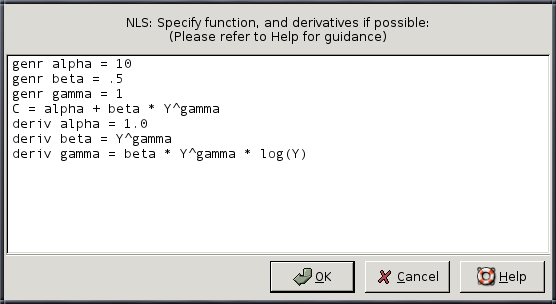
\includegraphics[scale=0.5]{figures/nls_window}
  \end{center}
\end{figure}


\section{Analytical and numerical derivatives}
\label{nls-deriv}

If you are able to figure out the derivatives of the regression
function with respect to the parameters, it is advisable to supply
those derivatives as shown in the examples above.  If that is not
possible, \app{gretl} will compute approximate numerical derivatives.
The properties of the NLS algorithm may not be so good in this case
(see Section \ref{nls-accuracy}).

If analytical derivatives are supplied, they are checked for
consistency with the given nonlinear function.  If the derivatives are
clearly incorrect estimation is aborted with an error message.  If the
derivatives are ``suspicious'' a warning message is issued but
estimation proceeds.  This warning may sometimes be triggered by
incorrect derivatives, but it may also be triggered by a high degree
of collinearity among the derivatives.

Note that you cannot mix analytical and numerical derivatives: you
should supply expressions for all of the derivatives or none.

\section{Controlling termination}
\label{nls-toler}

The NLS estimation procedure is an iterative process.  Iteration is
terminated when a convergence criterion is met or when a set maximum
number of iterations is reached, whichever comes first.  The maximum
number of iterations is \cmd{100*(k+1)} when analytical derivatives
are given and \cmd{200*(k+1)} when numerical derivatives are used,
where \verb+k+ denotes the number of parameters being estimated.  The
convergence criterion is that the relative error in the sum of
squares, and/or the relative error between the the coefficient vector
and the solution, is estimated to be no larger than some small value.
This ``small value'' is by default the machine precision to the power
3/4, but it can be set with the \cmd{genr} command using the special
variable \verb+toler+.  For example
\begin{code}
genr toler = .0001
\end{code}
 
will relax the tolerance to 0.0001.

\section{Details on the code}
\label{nls-code}

The underlying engine for NLS estimation is based on the \app{minpack}
suite of functions, available from
\href{http://www.netlib.org/minpack/}{netlib.org}.  Specifically, the
following \app{minpack} functions are called:

\begin{center}
  \begin{tabular}{ll}
    \verb+lmder+ & Levenberg--Marquandt algorithm with analytical
    derivatives
    \\
    \verb+chkder+ & Check the supplied analytical derivatives
    \\
    \verb+lmdif+ & Levenberg--Marquandt algorithm with numerical
    derivatives
    \\
    \verb+fdjac2+ & Compute final approximate Jacobian when using
    numerical derivatives
    \\
    \verb+dpmpar+ & Determine the machine precision
    \\
  \end{tabular}
\end{center}

On successful completion of the Levenberg--Marquandt iteration, a
Gauss--Newton regression is used to calculate the covariance matrix
for the parameter estimates.  Since NLS results are asymptotic, there
is room for debate over whether or not a correction for degrees of
freedom should be applied when calculating the standard error of the
regression (and the standard errors of the parameter estimates).  For
comparability with OLS, and in light of the reasoning given in
Davidson and MacKinnon (1993), the estimates shown in \app{gretl}
\emph{do} use a degrees of freedom correction.

\section{Numerical accuracy}
\label{nls-accuracy}

Table \ref{tab-nls} shows the results of running the \app{gretl} NLS
procedure on the 27 Statistical Reference Datasets made available by
the U.S.  National Institute of Standards and Technology (NIST) for
testing nonlinear regression software.\footnote{For a discussion of
  \app{gretl}'s accuracy in the estimation of linear models, see
  Appendix~\ref{app-accuracy}.}  For each dataset, two sets of
starting values for the parameters are given in the test files, so the
full test comprises 54 runs.  Two full tests were performed, one using
all analytical derivatives and one using all numerical approximations.
In each case the default tolerance was used.\footnote{The data shown
  in the table were gathered from a pre-release build of \app{gretl}
  version 1.0.9, compiled with \app{gcc} 3.3, linked against
  \app{glibc} 2.3.2, and run under Linux on an i686 PC (IBM ThinkPad
  A21m).}

Out of the 54 runs, \app{gretl} failed to produce a solution
in 4 cases when using analytical derivatives, and in 5 cases when
using numeric approximation. Of the four failures in analytical
derivatives mode, two were due to non-convergence of the
Levenberg--Marquandt algorithm after the maximum number of iterations
(on \verb+MGH09+ and \verb+Bennett5+, both described by NIST as of
``Higher difficulty'') and two were due to generation of range errors
(out-of-bounds floating point values) when computing the Jacobian (on
\verb+BoxBOD+ and \verb+MGH17+, described as of ``Higher difficulty''
and ``Average difficulty'' respectively).  The additional failure in
numerical approximation mode was on \verb+MGH10+ (``Higher
difficulty'', maximum number of iterations reached).

The table gives information on several aspects of the tests: the
number of outright failures, the average number of iterations taken to
produce a solution and two sorts of measure of the accuracy of the
estimates for both the parameters and the standard errors of the
parameters.

For each of the 54 runs in each mode, if the run produced a solution
the parameter estimates obtained by \app{gretl} were compared with the
NIST certified values.  We define the ``minimum correct figures'' for
a given run as the number of significant figures to which the
\emph{least accurate} \app{gretl} estimate agreed with the certified
value, for that run. The table shows both the average and the worst
case value of this variable across all the runs that produced a
solution.  The same information is shown for the estimated standard
errors.\footnote{For the standard errors, I excluded one outlier from
  the statistics shown in the table, namely \verb+Lanczos1+.  This is
  an odd case, using generated data with an almost-exact fit: the
  standard errors are 9 or 10 orders of magnitude smaller than the
  coefficients.  In this instance \app{gretl} could reproduce the
  certified standard errors to only 3 figures (analytical derivatives)
  and 2 figures (numerical derivatives).}  

The second measure of accuracy shown is the percentage of cases,
taking into account all parameters from all successful runs, in which
the \app{gretl} estimate agreed with the certified value to at least
the 6 significant figures which are printed by default in the
\app{gretl} regression output.

\begin{table}[htbp]
 \caption{Nonlinear regression: the NIST tests}
 \label{tab-nls}
  \begin{center}
    \begin{tabular}{lcc}
      � & \textit{Analytical derivatives} & \textit{Numerical derivatives}\\
        Failures in 54 tests & 4 & 5\\
        Average iterations & 32 & 127\\
        Mean of min. correct figures, & 8.120 & 6.980\\
        parameters \\
        Worst of min. correct figures, & 4 & 3\\
        parameters \\
        Mean of min. correct figures, & 8.000 & 5.673\\
        standard errors \\
        Worst of min. correct figures, & 5 & 2\\
        standard errors \\
        Percent correct to at least 6 figures, & 96.5 & 91.9\\
        parameters \\
        Percent correct to at least 6 figures, & 97.7 & 77.3\\
        standard errors \\
      \end{tabular}
    \end{center}
  \end{table}

  Using analytical derivatives, the worst case values for both
  parameters and standard errors were improved to 6 correct figures on
  the test machine when the tolerance was tightened to 1.0e$-$14.
  Using numerical derivatives, the same tightening of the tolerance
  raised the worst values to 5 correct figures for the parameters and
  3 figures for standard errors, at a cost of one additional failure
  of convergence.

  Note the overall superiority of analytical derivatives: on average
  solutions to the test problems were obtained with substantially
  fewer iterations and the results were more accurate (most notably
  for the estimated standard errors).  Note also that the six-digit
  results printed by \app{gretl} are not 100 percent reliable for
  difficult nonlinear problems (in particular when using numerical
  derivatives).  Having registered this caveat, the percentage of
  cases where the results were good to six digits or better seems high
  enough to justify their printing in this form.

%%% Local Variables: 
%%% mode: latex
%%% TeX-master: "gretl-guide"
%%% End: 
